
\begin{figure}[H]
  \centering
  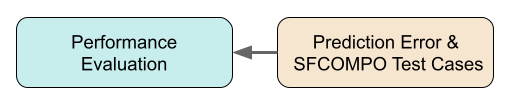
\includegraphics[width=0.7\linewidth]{./chapters/exp1/methodology4.png}
  \caption{Fourth portion of the flowchart from Figure \ref{fig:method} being 
           described in this section.}
\end{figure}

\subsection{Random Error Impacts on Prediction}
\label{sec:randerr}
As previously introduced in Section \ref{sec:testerr}, the prediction
performance is measured by evaluating the accuracy of the reactor type
classification or the error of the regression cases (burnup, \gls{U235}
enrichment, cooling time).  These performance metrics for all four prediction
types are compared across the three algorithms used: \textit{k}-nearest
neighbors (denoted in plots as \textit{kNN}), decision trees (denoted in plots
as \textit{Dec Tree} or \textit{DTree}), and \gls{MLL} calculations.  To judge
the degradation of predictions of the algorithms with increasing nuclide mass
measurement error (i.e., reduced information quality, detailed in section
\ref{sec:inforeduc1}), four plots are made with the introduced error on the
\textit{x}-axis and a prediction performance metric on the \textit{y}-axis.
Shown in Figure \ref{fig:randerr}, the \textit{y}-axis is always oriented so
that lower is poorer performance and higher is better performance. This is why
Figures \ref{fig:randerrB}--\ref{fig:randerrD} present a negative error on the
\textit{y}-axis.
\todo[inline]{In order to have consistency in plot presentation w future plots,
the plots in this section have a small delta-x to show error bars that are
otherwise hard to see.  Since the x-axis is continuous, this may force a return
to using the fill-between to visualize error bands instead.}

Figure \ref{fig:randerrA} shows the balanced accuracy of reactor type
classification, where a score of $1$ is perfect prediction and a score of $0$
is random classification. The error bars reflect a 99\% confidence interval.
While the two scikit-learn algorithms follow a very similar path of decreased
accuracy as the error increases, the \gls{MLL} calculation approach appears to
be more robust to the nuclide mass measurement error. This behavior is seen in
all four plots in Figure \ref{fig:randerr}. Another interesting result is that
the \gls{MLL} calculation performs slightly worse for low errors. If the
expected measurement errors of nuclide masses in a training database or in a
test sample can be guaranteed to be better than ~2\%, the \gls{MLL} calculation
is no longer the obvious preferred choice for reactor type prediction.

Although the balanced accuracy score provides slightly better information about
classification performance for an imbalanced data set (the training set is
26.8\% \gls{PWR}, 71.6\% \gls{BWR}, and 1.5\% \gls{PHWR}), it still does not
provide much detail about what is being misclassified. To probe this further,
Figure \ref{fig:cm_nuc29} shows two sets of confusion matrices.  The diagonal
squares are the fraction of true positives for each reactor type, where the
predicted label (\textit{x}-axis) is equal to the true label (\textit{y}-axis).
The off diagonal squares are the fraction of false positives for each reactor
type, where the predicted label is something other than the true label. In
addition to the numbers being included in the matrices, a colorbar provides
perceptially uniform shading for these true positive and false positive
fractions. 

In Figure \ref{fig:cm_nuc29_01}, the three algorithms are presented for the 1\%
random error case. In Figure \ref{fig:randerrA}, one can see these three data
points on the plot clustered near the top showing almost-perfect performance.
(A reminder that the true positive fractions in the confusion matrices do not
map directly to the balanced accuracy score, which puts more weight on the
underrepresented classes.) The confusion matrices give more dimension to this
near-perfect reactor type classification performance. The majority of the
misclassification is in \gls{PWR}s being classified as \gls{BWR}s: 0.4\% for
\textit{k}-nearest neighbors and decision trees, and 1.6\% for \gls{MLL}
calculations. Although, there are also some \gls{BWR}s that are misclassified
as \gls{PWR}s: 0.1\% for \textit{k}-nearest neighbors and decision trees, and
0.5\% for \gls{MLL} calculations. The \gls{PWR}/\gls{BWR} distinction is known
to be a difficult problem\todo{find citation}, so the correct \gls{PHWR}
classifications are not particularly notable for this discussion.

Figure \ref{fig:cm_nuc29_10} shows confusion matrices for the three algorithms
for the 10\% random error case. In Figure \ref{fig:randerrA}, one can see these
three data points on the plot, where the \gls{MLL} point is near a balanced
accuracy score of 1, and the scikit-learn algorithms both have score of around
0.93. As with the 1\% error case, the majority of the misclassification is in
\gls{PWR}s being classified as \gls{BWR}s: 11.0\% for \textit{k}-nearest
neighbors, 10.3\% for decision trees, and 1.7\% for \gls{MLL} calculations.
The \gls{BWR}s are being misclassified as \gls{PWR}s at the following
percentages: 3.4\% for \textit{k}-nearest neighbors, 3.7\% for decision trees,
and 0.5\% for \gls{MLL} calculations. Note how the performance of the \gls{MLL}
calculations are nearly the same for both error levels, which is shown by the 
\gls{MLL} line in Figure \ref{fig:randerrA}.

\todo[inline]{update with single confusion matrix grid and add 20\% conf matrix discussion}

Figure \ref{fig:randerrB} demonstrates the burnup prediction performance.  As
mentioned, the \textit{x}-axis is negative \gls{MAPE} so that higher is always
better.  The error bars reflect one standard deviation of the average
percentage errors.  Again, the \gls{MLL} method is robust to training set error
but performs slightly worse at low error values.  All three methods calculate
burnup with a maximum error of 5\% at 20\% error in the training set.  While it
is difficult to draw a baseline, this minimum performance level can serve as a
benchmark for the work presented in Chapter \ref{ch:exp2}. 

\begin{figure}[!hbt]
  \centering
  \begin{subfigure}[b]{0.49\textwidth}
    \centering
    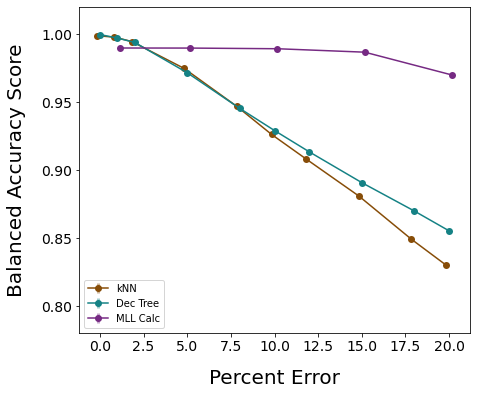
\includegraphics[width=\textwidth]{./chapters/exp1/randerr_compare_nuc29_BalAcc_rxtr.png}
    \caption{Balanced accuracy of reactor type classification with respect 
             to random error.}
    \label{fig:randerrA}
  \end{subfigure}
  \hfill
  \begin{subfigure}[b]{0.49\textwidth}
    \centering
    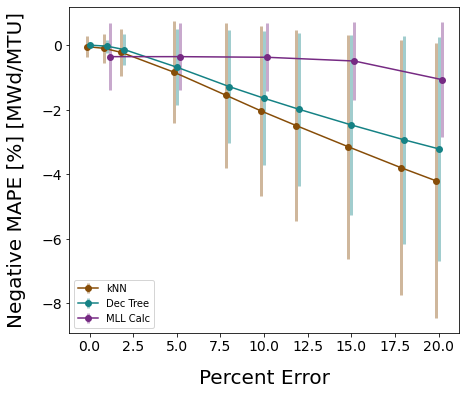
\includegraphics[width=\textwidth]{./chapters/exp1/randerr_compare_nuc29_MAPE_burn.png}
    \caption{Negative \gls{MAPE} of burnup regression with respect to 
             random error.}
    \label{fig:randerrB}
  \end{subfigure}
  \vskip\baselineskip
  \begin{subfigure}[b]{0.49\textwidth}
    \centering
    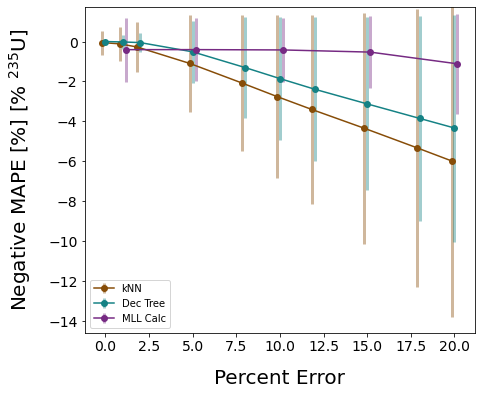
\includegraphics[width=\textwidth]{./chapters/exp1/randerr_compare_nuc29_MAPE_enri.png}
    \caption{Negative \gls{MAPE} of \gls{U235} enrichment regression with 
             respect to random error.}
    \label{fig:randerrC}
  \end{subfigure}
  \hfill
  \begin{subfigure}[b]{0.49\textwidth}
    \centering
    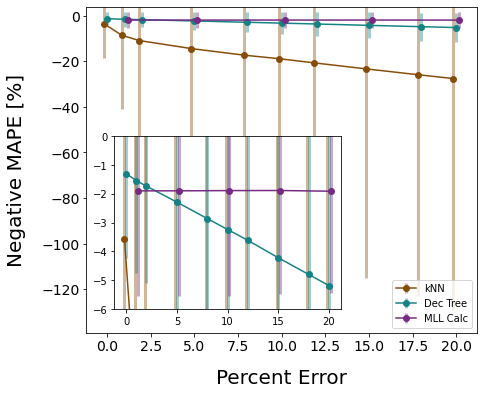
\includegraphics[width=\textwidth]{./chapters/exp1/randerr_compare_nuc29_MAPE_cool.png}
    \caption{Negative \gls{MAPE} of time since irradiation regression with 
             respect to random error.} 
    \label{fig:randerrD}
  \end{subfigure}
  \caption{Prediction performance of reactor type, burnup, enrichment, and 
           time since irradiation with respect to decreasing information
           quality in the form of uniform/random error applied to the nuclide 
           mass measurements in the training set.}
  \label{fig:randerr}
\end{figure}

\begin{figure}[!htb]
  \centering
  \begin{subfigure}[b]{\textwidth}
    \centering
    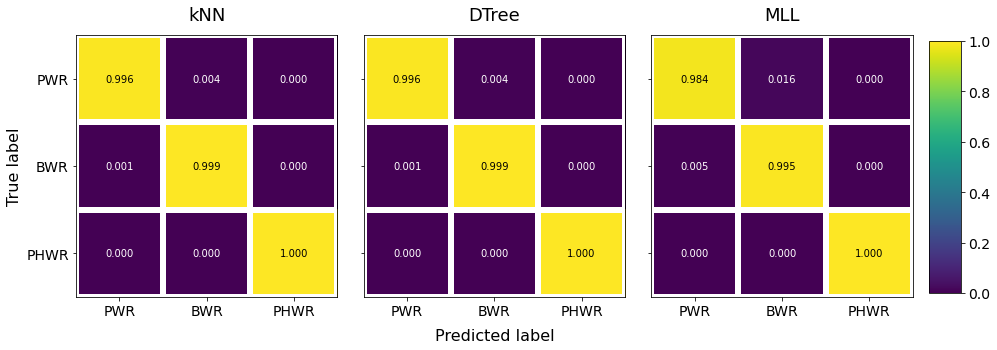
\includegraphics[width=\textwidth]{./chapters/exp1/confusion_matrix_nuc29_err01.png}
    \caption{Confusion matrices for 1\% error for each algorithm.}
    \label{fig:cm_nuc29_01}
  \end{subfigure}
  \vskip\baselineskip
  \begin{subfigure}[b]{\textwidth}
    \centering
    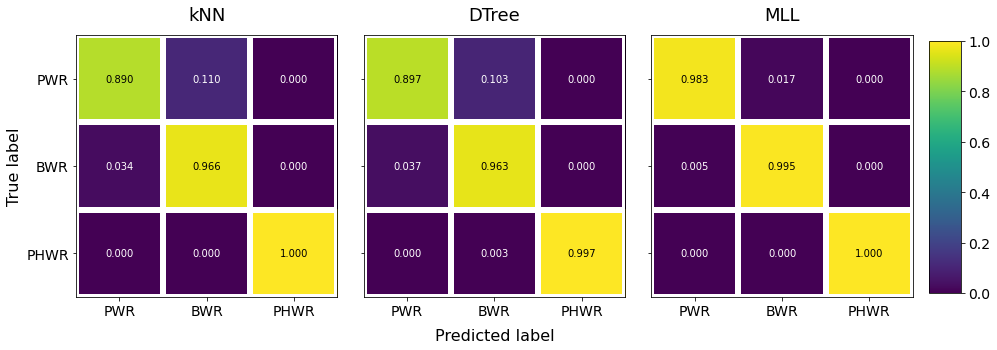
\includegraphics[width=\textwidth]{./chapters/exp1/confusion_matrix_nuc29_err10.png}
    \caption{Confusion matrices for 10\% error for each algorithm.}
    \label{fig:cm_nuc29_10}
  \end{subfigure}
  \vskip\baselineskip
  \begin{subfigure}[b]{\textwidth}
    \centering
    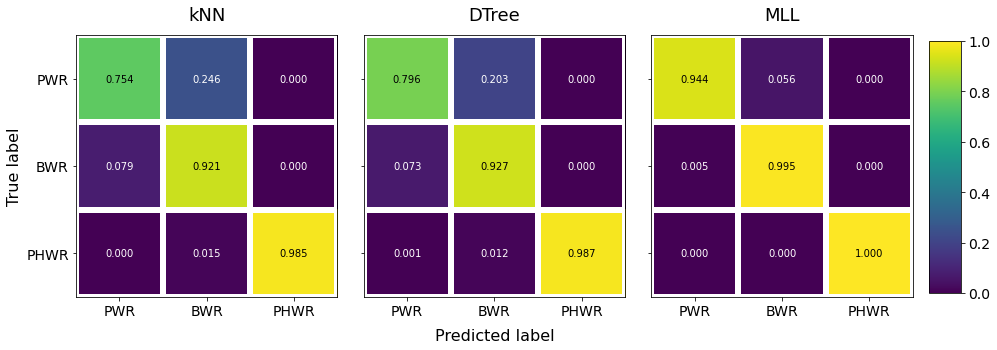
\includegraphics[width=\textwidth]{./chapters/exp1/confusion_matrix_nuc29_err20.png}
    \caption{Confusion matrices for 20\% error for each algorithm.}
    \label{fig:cm_nuc29_20}
  \end{subfigure}
  \caption{Confusion matrices for reactor type prediction for each algorithm 
           at three training set error levels: 1\%, 10\%, and 20\%.}
  \label{fig:cm_nuc29}
\end{figure}

Figure \ref{fig:randerrC} shows the trend of \gls{U235} enrichment prediction
with increasing error in the nuclide mass training set.  The error bars reflect
one standard deviation of the average percentage errors, and the behavior of
the \gls{MLL} method in Figure \ref{fig:randerrB} versus the scikit-learn
algorithms is the same here.  The maximum \gls{MAPE} is about 6\% at 20\%
training set error. 

Last, the time since irradiation prediction performance for the three
algorithms with respect to increasing nuclide mass error is pictured in Figure
\ref{fig:randerrD}.  The error bars reflect one standard deviation of the
average percentage errors.  The behavior of \textit{k}-nearest neighbors is
unique here versus the previous two regression categories; whereas the maximum
prediction \gls{MAPE}s remain under about 6\% for both the decision tree and
\gls{MLL} methods, the maximum error of \textit{k}-nearest neighbors reaches
nearly 30\% at 20\% nuclide mass error. \todo[inline]{1. do I need more ticks
on these y-axes?  2. I'm not sure why this is the case, and have not found a
way to figure this out yet. In previous iterations of the experiment, all
methods performed worse on the cooling time.  But now that is not the case and
it's only kNN performing significantly worse} 


\subsubsection{Model Generalization}
\label{sec:randerrC}

Although a key takeaway from Section \ref{sec:randerr} is that the \gls{MLL}
calculations are the most resilient to introduced error in the training set
features for all four prediction categories, there is another aspect of the
algorithm performance not explicitly shown in those plots: generalization.
\Gls{MLL} does not generalize to unseen data; it provides predictions based on
finding the closest training set entry to the test sample.  It (usually)
outperforms the scikit-learn methods in part because the training set is so
large. This is also true for the \textit{k}-nearest neighbor implementations
where $k=1$ (burnup and cooling time, as seen in Table \ref{tbl:exp1hypparam}).

\begin{figure}[!htb]
  \centering
  \begin{subfigure}[b]{0.495\textwidth}
    \centering
    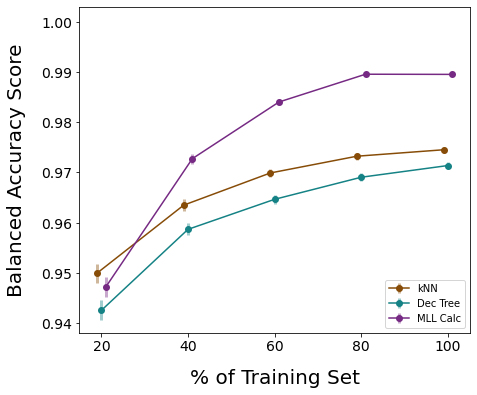
\includegraphics[width=\textwidth]{./chapters/exp1/learncurve_nuc29_err05_BalAcc_rxtr.png}
    \caption{Balanced accuracy of reactor type classification with respect 
             to training set size.}
    \label{fig:learnsA}
  \end{subfigure}
  \hfill
  \begin{subfigure}[b]{0.485\textwidth}
    \centering
    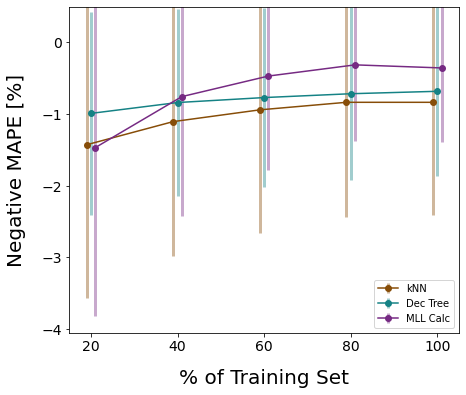
\includegraphics[width=\textwidth]{./chapters/exp1/learncurve_nuc29_err05_MAPE_burn.png}
    \caption{Negative \gls{MAPE} of burnup regression with respect to 
             to training set size.}
    \label{fig:learnsB}
  \end{subfigure}
  \vskip\baselineskip
  \begin{subfigure}[b]{0.48\textwidth}
    \centering
    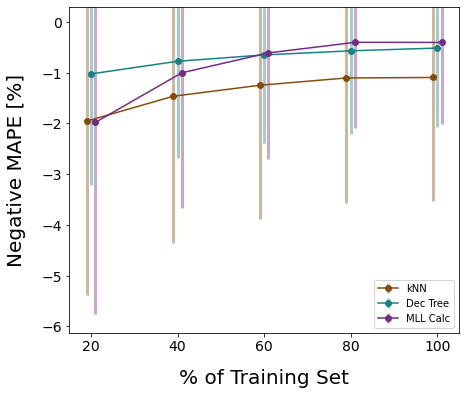
\includegraphics[width=\textwidth]{./chapters/exp1/learncurve_nuc29_err05_MAPE_enri.png}
    \caption{Negative \gls{MAPE} of \gls{U235} enrichment regression with 
             respect to training set size.}
    \label{fig:learnsC}
  \end{subfigure}
  \hfill
  \begin{subfigure}[b]{0.50\textwidth}
    \centering
    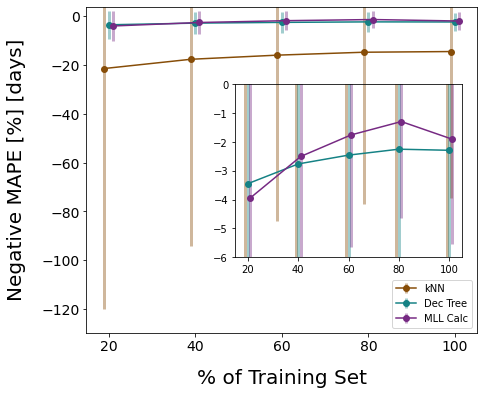
\includegraphics[width=\textwidth]{./chapters/exp1/learncurve_nuc29_err05_MAPE_cool.png}
    \caption{Negative \gls{MAPE} of time since irradiation regression with 
             respect to training set size.}
    \label{fig:learnsD}
  \end{subfigure}
  \caption[Learning curves for all four prediction parameters]
          {Learning curves for reactor type, burnup, enrichment, and time 
           since irradiation with respect to increasing fraction of the 
           training set, for 5\% training set random error.}
  \label{fig:learns}
\end{figure}

One way to show that an algorithm is generalizing well in comparison to others
is to view the shape of its learning curve (introduced in Section
\ref{sec:complexity}): the prediction performance with respect to training set
size.  It is crucial to have the training sets be identical for each algorithm,
so they were created in advance and the learning curves are constructed
manually rather than relying on the scikit-learn method.  Smaller training sets
were created from the original one by taking 80\%, 60\%, 40\%, and 20\% of the
entries. The training sets are all stratified so that the original fractions of
\gls{BWR}, \gls{PWR}, and \gls{PHWR} are retained. They are also built on top
of one another, so the 20\%-size training set is contained within the 40\%-size
set, and so forth.

Learning curves were constructed for all four prediction categories,
demonstrated in Figure \ref{fig:learns}. As in Figures
\ref{fig:randrxtr}--\ref{fig:randcool} , the vertical axis is always oriented
so that lower is poorer performance and higher is better performance; also, the
error bars reflect a 99\% confidence interval for Figure \ref{fig:learnsA}, and
one standard deviation of the average percentage errors for Figures
\ref{fig:learnsB}--\ref{fig:learnsD}.  These learning curves represent the 5\%
random error case in Figures \ref{fig:randrxtr}--\ref{fig:randcool}, so the
scores/errors in these figures are the data points at the 100\% training set
level in Figure \ref{fig:learns}.  Therefore, the leftmost data in Figure
\ref{fig:learns} will show the \gls{MLL} point being slightly above the
scikit-learn points for the reactor type, burnup, and enrichment predictions,
and the \textit{k}-nearest neighbor point is below the \gls{MLL} and decision
trees points for time since irradiation.  

Figure \ref{fig:learnsA} shows that the balanced accuracy score of reactor type
classification for the \gls{MLL} calculations decreases more at lower training
set size than for the scikit-learn algorithms. Here, the curve crosses below
the \textit{k}-nearest neighbors curve at the lowest training set size of 20\%.
For the burnup \gls{MAPE} in Figure \ref{fig:learnsB} and the enrichment
\gls{MAPE} in Figure \ref{fig:learnsC}, the \gls{MLL} curve crosses below both
of the scikit-learn algorithm curves. This happens between 20\% and 40\%
training set size for burnup, and between 40\% and 60\% training set size for
enrichment.  Lastly, Figure \ref{fig:learnsD} shows a different arrangement,
which is to be expected from the results shown in Figure \ref{fig:randcool},
where the \textit{k}-nearest neighbors performance is significantly worse than
the other two algorithms. Because the \textit{k}-nearest neighbors curve and
error bars are so large, there is an inset showing a closeup of the other two
curves above -6\%.  The decision trees and \gls{MLL} calculations curves now
appear to follow the trend in the burnup and enrichment cases, and the
\gls{MLL} curve crosses under the decision trees curve between 20\% and 40\%
training set size.  

There is a dependence on training set size for all three algorithms in Figure
\ref{fig:learns}. For the most part, the \textit{k}-nearest neighbors and
decision trees curves follow an approximately parallel path, whereas the
\gls{MLL} method shows an increased rate of degradation at low training set
sizes. Since this training set is large enough, i.e., the prediction parameters
were included in small enough steps, that \gls{MLL} has consistent performance
at the larger sizes, there is not a concern in this work about its inability to
generalize. It must be noted, however, that the \gls{MLL} approach requires a
fine grid of simulation parameters in a training database to perform better
than the simple scikit-learn algorithms.

\subsubsection{Reactor Type Prior Knowledge}
\label{sec:randerrD}

There is similar work being done to this work that focuses on similar
prediction categories but in a serial manner, i.e., first determining the
reactor type before moving forward with other predictions \cite{serial_ml}.
This work predicts reactor operation parameters while blind to the reactor
type, but it makes sense intuitively that having previous knowledge of the
reactor type would allow more accurate regression of these parameters.
Therefore, the change in regression performance from the reactor type-blind
predictions to having prior knowledge of the reactor type is discussed.

The workflow was repeated for the three regression cases where they were
trained on reactor type-specific training sets. A 5\% random error was applied
to these training sets, and the 5\% random error full training set was used as
comparison. The errors for each algorithm (\textit{k}-nearest neighbors,
decision trees, and \gls{MLL} calculations) were tallied for each regression
category (burnup, enrichment, and time since irradiation) and within that, for
each reactor type (\gls{PWR}, \gls{BWR}, \gls{PHWR}). Two sets of error were
tracked: whether the reactor type was \textit{known} or \textit{unknown} prior
to prediction.

Table \ref{tbl:knownrxtr} shows the \gls{MAPE}s for each regression category
and within that, for each reactor type (\gls{PWR}, \gls{BWR}, \gls{PHWR}).  The
columns are separated first by the algorithms and second by whether the reactor
type was known or unknown prior to prediction, denoted as \textit{K} and
\textit{U}, respectively. Most of these relative errors are quite low, and
around or under 2\%.  So, e.g., despite burnup prediction from \glspl{PHWR}s
improving, it was by 0.61\%, a precision of which may not be of concern. Still,
these performance differences can be looked at in more detail.  

\begin{table}[!htb]
  \centering
  \begin{tabular}{@{}llllllll@{}}
    \toprule
    &  &  \multicolumn{2}{c}{\textit{k}NN} 
    &     \multicolumn{2}{c}{Dec Trees} 
    &     \multicolumn{2}{c}{MLL Calcs} \\ 
    \toprule
    \begin{tabular}[c]{@{}l@{}}Prediction\\ Parameter\end{tabular} &
    \begin{tabular}[c]{@{}l@{}}Reactor \\ Type\end{tabular} &
    K & U &  K & U & K & U \\ \midrule
    \multirow{3}{*}{\begin{tabular}[c]{@{}l@{}}Burnup \\ \% {$[MWd/MTU]$} \end{tabular}}
     & PWR  & 0.60  & 0.66  & 0.54 & 0.75 & 0.24 & 0.25 \\
     & BWR  & 0.88  & 0.90  & 0.60 & 0.66 & 0.40 & 0.40 \\
     & PHWR & 0.66  & 1.27  & 0.14 & 0.54 & 0.28 & 0.28 \\ \hline
    \multirow{3}{*}{\begin{tabular}[c]{@{}l@{}}Enrichment \\ \% {$[\%\:{}^{235}\text{U}]$} \end{tabular}}
     & PWR  & 0.85  & 0.99  & 0.36 & 0.48 & 0.26 & 0.29 \\
     & BWR  & 1.14  & 1.16  & 0.51 & 0.54 & 0.45 & 0.46 \\
     & PHWR & 0.00  & 0.00  & 0.00 & 0.02 & 0.00 & 0.00 \\ \hline
    \multirow{3}{*}{\begin{tabular}[c]{@{}l@{}}Time Since \\ Irradiation \\ \% {$[days]$} \end{tabular}}
     & PWR  & 11.44 & 10.48 & 2.35 & 2.19 & 1.55 & 1.46 \\
     & BWR  & 15.39 & 15.48 & 2.27 & 2.28 & 2.06 & 2.05 \\
     & PHWR & 19.32 & 34.41 & 4.96 & 4.52 & 2.30 & 2.30 \\ \bottomrule
  \end{tabular}
  \caption[\acrshort{MAPE}s for three regression cases comparing known versus 
           unknown reactor type prior knowledge]
          {\acrshort{MAPE}s for the three prediction cases for each algorithm 
           at 5\% training set error. \textit{K} refers to \textit{known} 
           reactor type and \textit{U} refers to \textit{unknown} reactor type 
           prior to regression.}
  \label{tbl:knownrxtr}
\end{table}

To better see these performance differences, the percent change in prediction
\gls{MAE} for each algorithm and reactor type between the reactor type being
known versus unknown prior to prediction was calculated as: $100 \cdot
\frac{MAE_{unknown} - MAE_{known}}{MAE_{unknown}}$.  This was chosen to be
relative to the unknown error since that is the benchmark in this case.  Figure
\ref{fig:knownrxtr} is three heatmaps that show this percent change for each
prediction category, algorithm, and reactor type.  This value is reflected by a
diverging color bar as well as a positive or negative percentage in each
square.  The positive percentages indicate the error decreased/improved from
the unknown reactor type case to the known reactor type case.  The negative
percentages indicate the error increased/worsened from the unknown to the known
case. 

\begin{figure}[!htb]
  \centering
  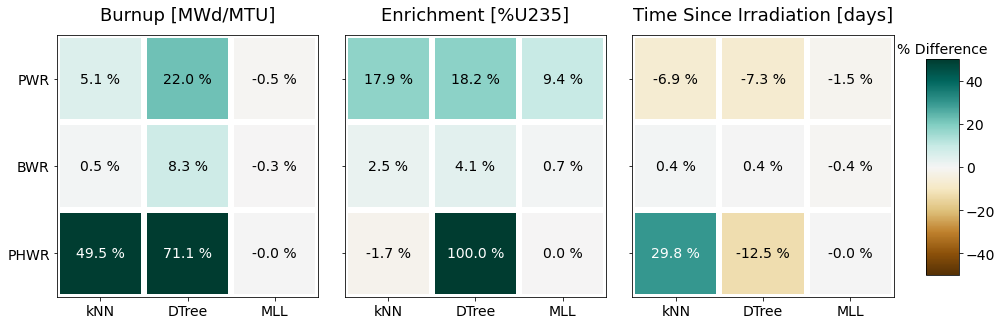
\includegraphics[width=\textwidth]{./chapters/exp1/rxtr-type_known-unknown_diff_err05.png}
  \caption[Heatmaps for three regression cases comparing known versus 
           unknown reactor type prior knowledge]
          {Heatmaps for the three regression cases showing the percent 
           difference in prediction error between a known reactor type 
           and unknown reactor type using a 5\% training set error.}
  \todo[inline]{would this be better shown with a plot that has little arrows? or leave like this?}
  \label{fig:knownrxtr}
\end{figure}

For burnup prediction, most differences are within $\pm10\%$ except for three
scenarios.  The decision tree algorithm has improved burnup prediction for
\glspl{PWR}s by 22.0\% and for \glspl{PHWR}s by 71.1\% given a known reactor
type.  The \textit{k}-nearest neighbors algorithm has 49.5\% improved burnup
prediction for the \gls{PHWR}. For \gls{U235} enrichment, the \gls{PWR}
predictions improve by approximately 18\% for the scikit-learn algorithms.
Even though the value is within $\pm10\%$, this is the only scenario where
there is an appreciable difference in \gls{MLL} performance. The decision tree
enrichment prediction of \glspl{PHWR}s also has a sizeable improvement of
100.0\%.  The time since irradiation predictions for the most part do not show
improvement outside of $\pm10\%$. Of note is some volatile behavior for the
\gls{PHWR} case with the scikit-learn algorithms.  While \textit{k}-nearest
neighbors improves by 29.8\%, the decision tree predictions were worse by
12.5\%.  Since the main concern here is showing how prediction performance
improves with prior reactor type knowledge, this reduction in performance is
odd but not worthy of further investigation.

The improvements in the \gls{PHWR} predictions are not surprising since the
generalization of the scikit-learn algorithms could lead to the unique
\gls{PHWR} cases being ignored, since they are after all only 1.5\% of the
training set.  Another interesting result is that the \gls{BWR} predictions
experience no large changes, which makes sense given that they comprise 72\% of
the training set. Also, the \gls{MLL} predictions are approximately the same,
which is expected because this algorithm does not generalize, and the
prediction comes as a set of labels and is therefore already linked to the
reactor type. Overall, it is important to be aware that the regression labels
coming from a \gls{PHWR} will be unlikely to be optimal results (except for
those from \gls{MLL} calculations).

%\begin{table}[!htb]
%  \centering
%  \begin{tabular}{@{}llllllll@{}}
%    \toprule
%    &  &  \multicolumn{2}{c}{\textit{k}NN} 
%    &     \multicolumn{2}{c}{Dec Trees} 
%    &     \multicolumn{2}{c}{MLL Calcs} \\ 
%    \toprule
%    \begin{tabular}[c]{@{}l@{}}Prediction\\ Parameter\end{tabular} &
%    \begin{tabular}[c]{@{}l@{}}Reactor \\ Type\end{tabular} &
%    K & U &  K & U & K & U \\ \midrule
%    \multirow{3}{*}{\begin{tabular}[c]{@{}l@{}}Burnup \\ \% {$[MWd/MTU]$} \end{tabular}}
%     & PWR  & 0.08  & 0.08  & 0.03 & 0.04 & 0.24 & 0.25 \\ 
%     & BWR  & 0.11  & 0.10  & 0.03 & 0.03 & 0.40 & 0.40 \\ 
%     & PHWR & 0.13  & 0.19  & 0.01 & 0.03 & 0.29 & 0.29 \\ \hline
%    \multirow{3}{*}{\begin{tabular}[c]{@{}l@{}}Enrichment \\ \% {$[\%\:{}^{235}\text{U}]$} \end{tabular}}
%     & PWR  & 0.10  & 0.11  & 0.02 & 0.02 & 0.26 & 0.29 \\ 
%     & BWR  & 0.12  & 0.12  & 0.02 & 0.02 & 0.46 & 0.46 \\ 
%     & PHWR & 0.00  & 0.00  & 0.00 & 0.00 & 0.00 & 0.00 \\ \hline
%    \multirow{3}{*}{\begin{tabular}[c]{@{}l@{}}Time Since \\ Irradiation \\ \% {$[days]$} \end{tabular}}
%     & PWR  & 6.47  & 6.13  & 1.50 & 1.43 & 1.55 & 1.46 \\ 
%     & BWR  & 9.18  & 9.15  & 1.56 & 1.53 & 2.07 & 2.05 \\ 
%     & PHWR & 13.78 & 18.62 & 4.51 & 3.71 & 2.30 & 2.30 \\ \bottomrule
%  \end{tabular}
%  \caption{\gls{MAPE}s for the three prediction cases for each algorithm at 1\% 
%           training set error. \textit{K} refers to \textit{known} reactor 
%           type and \textit{U} refers to \textit{unknown} reactor type prior 
%           to regression.}
%  \label{tbl:knownrxtr}
%\end{table}

%\begin{figure}[!htb]
%  \centering
%  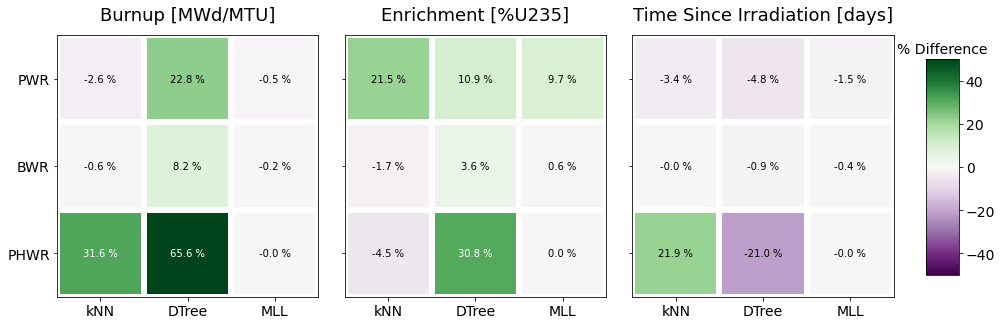
\includegraphics[width=\textwidth]{./chapters/exp1/rxtr-type_known-unknown_diff_err01.png}
%  \caption{Heatmaps for the three regression cases showing the percent 
%           difference in prediction error between a known reactor type 
%           and unknown reactor type.}
%  \label{fig:knownrxtr}
%\end{figure}



\subsection{SFCOMPO Test Set}
\label{sec:sfcompo}

\todo[inline]{1. all of my commentary on performance improvement for the
sfcompo test set is outlined to go into the future work section. or should it
go here?  2. also, there may be some useful information from the model
generalization or rxtr type prior knowledge sections that could be useful here
for more in depth discussion. 3. this ended up really motivating the use of
relative error versus absolute (really, both) so it could maybe go first, then
the random error results section could go second using the relative error
plots?}

The testing described in Section \ref{sec:randerr} describes the process of
evaluating the methodology with test cases drawn from the training database.
It is also helpful to test the methodology against real assays of \gls{SNF}.
The \gls{SFCOMPO} database was created to allow access to these sorts of
measurements linked to the reactor operation parameters being predicted in this
work. \cite{sfcompo}. The only parameter not part of the \gls{SFCOMPO} database
is the time since irradiation, so that is not predicted here. 

\begin{figure}[!htb]
  \centering
  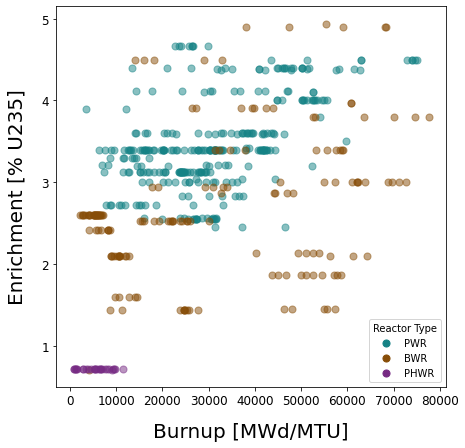
\includegraphics[width=0.7\textwidth]{./chapters/exp1/sfcompo_scatter_viz.png}
  \caption{Scatter plot showing the range of reactor operation parameters in 
           the \gls{SFCOMPO} testing set that are being predicted.}
  \label{fig:sfcoscatter}
  \todo[inline]{maybe show comparison against training E v B scatter plot}
\end{figure}

There are 505 test cases that are able to be compared against the training
database.  The number of each reactor type is as follows: 312 \gls{PWR}s, 165
\gls{BWR}s, and 28 \gls{PHWR}s. The space of enrichment and burnup values is
visualized in Figure \ref{fig:sfcoscatter}. These are sufficiently represented
in the training set design, as pictured in Figure \ref{fig:trainhist}, although
the proportions of \gls{PWR} and \gls{BWR} are approximately opposite to the
training set. The assays in \gls{SFCOMPO} are presented as nuclide
concentrations with the units \textit{milligrams per grams of initial uranium},
or $mg/gU_i$. The training set of nuclide measurements in \textit{grams} is
converted to these concentration units prior to prediction is converted to
these concentration units prior to prediction. 

There is one main issue with using \gls{SFCOMPO} as a testing set: missing
nuclide measurements.  The feature set of 29 nuclides in Table
\ref{tbl:nucmass} was chosen based on the frequency of these measurements being
present in the database at an arbitrary level of 100 measurements. This
happened before filtering, so there are some nuclide measurements present at
under 100 counts.  Each nuclide's frequency in \gls{SFCOMPO} is listed in Table
\ref{tbl:missing}.  While every assay contains several plutonium measurements
and most contain uranium measurements as well, the remaining nuclides are
present at a much lower rate. 

\begin{table}[!htb]
  \centering
  \begin{tabular}{>{\raggedleft}m{0.6in}
                                m{0.4in}
                  >{\raggedleft}m{0.6in}
                                m{0.4in}
                  >{\raggedleft}m{0.6in}
                                m{0.4in}}
    \toprule
    \rowcolor[gray]{0.88} am241  & 237 & nd145 & 162 & sm147 & 97  \\  
    \rowcolor[gray]{0.95} am242m & 110 & nd146 & 139 & sm149 & 97  \\ 
    \rowcolor[gray]{0.88} am243  & 203 & nd148 & 275 & sm150 & 97  \\ 
    \rowcolor[gray]{0.95} cm242  & 214 & nd150 & 121 & sm151 & 97  \\ 
    \rowcolor[gray]{0.88} cm244  & 269 & np237 & 155 & sm152 & 97  \\ 
    \rowcolor[gray]{0.95} cs134  & 113 & pu238 & 369 & u234  & 355 \\ 
    \rowcolor[gray]{0.88} cs137  & 185 & pu239 & 505 & u235  & 479 \\ 
    \rowcolor[gray]{0.95} eu154  & 100 & pu240 & 505 & u236  & 462 \\ 
    \rowcolor[gray]{0.88} nd143  & 162 & pu241 & 504 & u238  & 433 \\ 
    \rowcolor[gray]{0.95} nd144  & 113 & pu242 & 505 &       &     \\ \bottomrule
  \end{tabular}
  \caption{Number of assays each nuclide is measured for in the \gls{SFCOMPO}
           database.}
  \label{tbl:missing}
\end{table}

Although some algorithms in theory can handle null values in the training
stage, scikit-learn does not currently include this capability. The \gls{MLL}
method is designed to handle null values, however. This is done by converting
them to zero and filtering out all zero-valued nuclides during the likelihood
calculations. But there is a technique more commonly applied than converting
missing values to zero: imputation. This involves taking the mean or median of
the existing features and applying that value to the assays in which it is
missing.  The remainder of this section dicusses using the three algorithms to
predict the \gls{SFCOMPO} test cases where the nulls are both converted to zero
and imputed using the mean.  \todo[inline]{is converting to zero technically
imputation as well?}

\subsubsection{Reactor Type Classification}

Table \ref{tbl:sfcorxtr} presents two metrics for the two missing value
techniques: the accuracy and balanced accuracy scores. The accuracy scores for
both the imputed nulls and zero-nulls test sets are mostly under 0.62, which is
the fraction of \gls{PWR} entries.  Therefore, a classifier could predict
\gls{PWR} every time and do better than these accuracy scores.  For the
zero-nulls test set predictions using \gls{MLL}, however, the accuracy of 0.72
does exceed the "majority guess" accuracy of 0.62.  Since \gls{MLL}
calculations filter out null values, it is expected that the scores will be
higher for all prediction categories where \gls{MLL} is being used with the
zero-nulls test set. This expected \gls{MLL} performance also holds true when
looking at the balanced accuracy score.  A balanced accuracy score of 0 denotes
random guessing, but it can also be negative if the classifications are worse
than random guessing. The balanced accuracy of 0.63 for the zero-nulls case is
a promising result. The balanced accuracies of \textit{k}-nearest neighbors and
decision trees are all quite low. Also, the higher accuracies correspond to lower
balanced accuracies, and vice versa. Therefore, further investigation is
necessary.

\begin{table}[!htb]
  \centering
  \begin{tabular}{@{}m{1.5in}llllll@{}}
    \toprule
    & \multicolumn{3}{m{2in}}{Accuracy Scores} 
    & \multicolumn{3}{l}{Balanced Accuracy Scores} \\ 
    \toprule
    Null Handling    & kNN   & DTree  & MLL   & kNN   & DTree  & MLL    \\ \midrule
    Imputed Nulls    & 0.52  & 0.60   & 0.39  & 0.09  & 0.12   & -0.01  \\
    Zero-value Nulls & 0.45  & 0.42   & 0.72  & 0.21  & 0.30   & 0.63   \\ \bottomrule
    \end{tabular}
  \caption{Accuracy and balanced accuracy scores for reactor type prediction 
           of the \gls{SFCOMPO} test cases.}
  \label{tbl:sfcorxtr}
\end{table}

\begin{figure}[!htb]
  \centering
  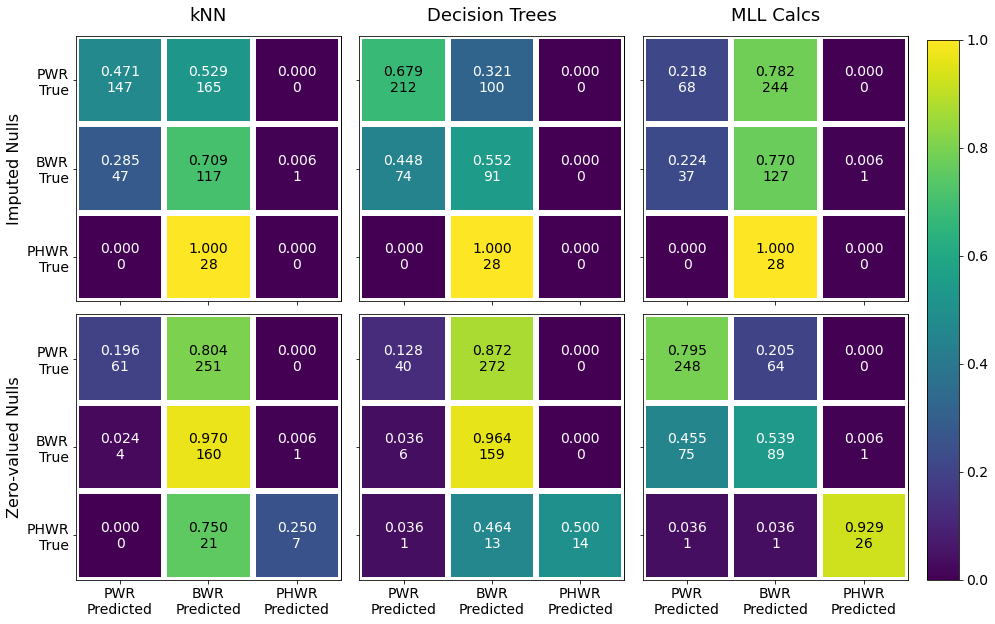
\includegraphics[width=\textwidth]{./chapters/exp1/confusion_matrix_sfco.png}
  \caption{Confusion matrices of reactor type prediction for each algorithm 
           using two missing entry techniques: imputation with mean values (top 
           panel) and replacement with zero (bottom panel).}
  \label{fig:cm}
\end{figure}

Figure \ref{fig:cm} allows for a deeper look into what is happening with the
reactor type predictions for both of the \gls{SFCOMPO} test sets.  The matrices
from using mean-imputed null values are in the top panel and the matrices from
using zero-filled null values are in the bottom panel.  The scikit-learn
algorithms have a higher accuracy for the imputed null values test set than
their zero-null values counterparts, but the balanced accuracies follow the
opposite direction. For \textit{k}-nearest neighbors, imputed nulls cause more
than half of the \gls{PWR}s and all of the \gls{PHWR}s to be misclassified as
\gls{BWR}s. Additionally, 28.5\% \gls{BWR}s are misclassified as \gls{PWR}s.
For the zero-nulls test set, there is a much larger correct \gls{BWR}
classification percentage, but also a much larger \gls{PWR} misclassification
percentage. The \gls{PHWR} true positive percentage increases from 0 to 25\%.
\Gls{BWR} (32\% of test cases) and \gls{PHWR} (5.5\% of test cases) are the two
minority classes in the database.  Because they both have higher true positive
fractions but there were overall fewer correct predictions (from a much higher
\gls{PWR} misclassification) from the imputed nulls to the zero-nulls, the
accuracy went down but the balanced accuracy went up.

Decision trees follows a similar pattern the the \textit{k}-nearest neighbors
example.  The \gls{PWR} misclassification increases from the imputed nulls to
the zero-nulls test set in a similar manner, although the original \gls{PWR}
true positive fraction is higher (leading to a higher accuracy for the imputed
nulls case).  As before, the \gls{BWR} correct classification increases
drastically from the imputed nulls to zero-nulls case.  Additionally, the
\gls{PHWR} classifiction improvement from imputed nulls to zero-nulls is better
for decision trees than for \textit{k}-nearest neighbors.  Therefore, again,
the accuracy decreased and the balanced accuracy increased. The larger
improvement for the minority classes has led to the larger balanced accuracy
improvement for decision trees.

In Figure \ref{fig:cm}, the confusion matrices for the \gls{MLL} calculations
tell a very different story than those for the scikit-learn algorithms.  The
only similarity is that using imputed nulls causes all \gls{PHWR}s to be
classified as \gls{BWR}s. \gls{PWR}s are misclassified as \gls{BWR}s at 78.2\%,
and \gls{BWR}s are misclassified as \gls{PWR}s at 22.4\%. For the zero-nulls
test set, \gls{PHWR}s and \gls{PWR}s true positive percentages sharply improve
to 92.9\% and 79.5\%, respectively.  The true positive rate for \gls{BWR}s,
however, decreases from 77.0\% to 53.9\%. This is the opposite trend from both
of the scikit-learn algorithms.  Despite the misclassification increase for
\gls{BWR}s, both the accuracy score and balanced accuracy score increase for
\gls{MLL} calculations when moving from using imputed null values to zero-null
values in the test set. The improvement in \gls{MLL} classification is likely
because the imputed nulls test set hides information rather than removing it
from consideration, which is what the zero-nulls test set does. 

All three algorithms using both test sets tend towards misclassifying
\gls{PHWR}s as \gls{BWR}s (except for \gls{MLL} calculations using zero-null
missing values).  This is likely because \gls{BWR}s comprise the majority of
the training set (72\%), and no matter how the missing measurements are handled
there may be too little information to predict these well with most algorithms.
For the two scikit-learn algorithms, the zero-nulls test set predicts
\gls{BWR}s the majority of the time (despite there being 50\% correct
\gls{PHWR} prediction for decision trees). This also is likely from \gls{BWR}
being the training set majority class, so with many nuclides measuring at zero,
there are likely to be few good matches, and the majority class becomes the
most likely prediction. This explanation is possibly applicable to the imputed
nulls test set as well, but the behavior pattern is less clear because the
imputed nulls give more information for these algorithms than zero-value nulls
(since the zero-values cannot be removed from consideration), so a larger
proportion of \gls{PWR}s are being predicted properly.  \todo[inline]{look up
paper that uses only U/Pu to predict, because that would be the only way these
505 cases would be able to be predicted without having so much missing
information. MLL essentially does this for 0 null case which is why it does
better than the rest}

\subsubsection{Regression Cases}

Next, the prediction of \gls{SFCOMPO} test samples for the regression cases
will be discussed. There is no time since irradiation value in the database, so
only burnup and \gls{U235} enrichment are discussed here.  While the mean and
median errors for burnup and enrichment prediction are listed in Tables
\ref{tbl:sfcoburn} and \ref{tbl:sfcoenri}, respectively, there are also box
plots inlcuded for both absolute and relative errors in Figures
\ref{fig:sfcoburn} and \ref{fig:sfcoenri}, respectively.  Box plots were chosen
since they can provide a larger amount of information than just a mean or
median value.  The white triangles represent the mean error, and the white line
in notched box is the median error. The box itself is the 25\% (Q1) and 75\%
(Q3) quartiles at the bottom and top, respectively. The error bars or whiskers
are meant to represent the spread of all errors minus the outliers.  The bottom
whisker reaches to $Q1 - 1.5*(Q3-Q1)$ and the top whisker reaches to $Q3 +
1.5*(Q3-Q1)$. Any values outside of this range are considered outliers.
\cite{matplotlib}

\noindent \textbf{Burnup}

The expected results that \gls{MLL} will perform better with the zero-nulls
test set also holds true for the regression cases, as shown in Table
\ref{tbl:sfcoburn}.  While the scikit-learn algorithms have a moderate increase
in both the mean and median burnup errors from the imputed nulls to the
zero-nulls, the \gls{MLL} calculations have an order of magnitude decrease in
error when moving in that same direction.  Seeing this trend between Figures
\ref{fig:burnimp} and \ref{fig:burn0} is a little difficult due to the
different ranges on the \textit{y}-axes, but the drastic improvement in
\gls{MLL} burnup error from the imputed nulls in Figure \ref{fig:burnimp} to
the zero-nulls in Figure \ref{fig:burn0} is still visually clear. In the latter
figure, there is one outlier for \textit{k}-nearest neighbors and 39 for
\gls{MLL} calculations.

\begin{table}[!htb]
  \centering
  \begin{tabular}{@{}m{1.5in}llllll@{}}
    \toprule
                     & \multicolumn{3}{m{2in}}{Mean Errors [GWd/MTU]} & \multicolumn{3}{c}{Median Errors [GWd/MTU]} \\ \toprule
    Null Handling    & kNN           & DTree         & MLL           & kNN            & DTree          & MLL    \\ \midrule
    Imputed Nulls    & 9.43          & 10.89         & 13.17         & 7.26           & 8.28           & 10.84  \\
    Zero-value Nulls & 14.88         & 15.18         & 3.53          & 11.47          & 8.79           & 1.70   \\ \bottomrule
  \end{tabular}
  \caption{Mean and median errors for burnup prediction of the \gls{SFCOMPO} 
           test cases.}
  \label{tbl:sfcoburn}
\end{table}

Although the mean and median errors are contained in the range of $1-15
GWd/MTU$, the large spread in burnup errors in Figures \ref{fig:burnimp} and
\ref{fig:burn0} for all three algorithms was broad enough to warrant an
investigation into the range of relative errors, expressed as percent errors in
Figures \ref{fig:burnimppct} and \ref{fig:burn0pct}.  In Figure
\ref{fig:burnimppct} there are 75, 72, and 73 outliers (all around 15\% of the
test database) for the \textit{k}-nearest neighbors, decision trees, and
\gls{MLL} calculations, respectively.  In Figure \ref{fig:burn0pct} there are
45 outliers for the \gls{MLL} calculations.

\begin{figure}[!htb]
  \centering
  \begin{subfigure}[b]{0.49\textwidth}
    \centering
    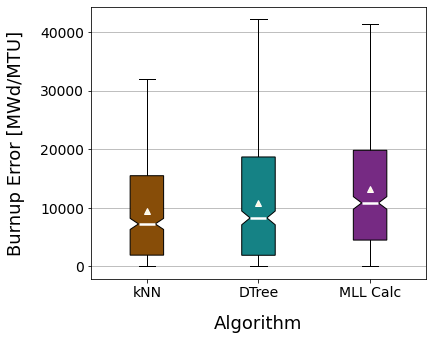
\includegraphics[width=\textwidth]{./chapters/exp1/sfcompo_boxplots_impnull_burn.png}
    \caption{Box plots of burnup errors using mean-imputed null values.}
    \label{fig:burnimp}
  \end{subfigure}
  \hfill
  \begin{subfigure}[b]{0.49\textwidth}
    \centering
    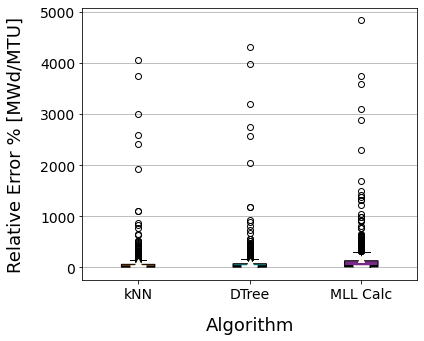
\includegraphics[width=\textwidth]{./chapters/exp1/sfcompo_boxplots_impnull_pcterr_burn.png}
    \caption{Box plots of burnup percentage errors using mean-imputed null values.}
    \label{fig:burnimppct}
  \end{subfigure}
  \vskip\baselineskip
  \begin{subfigure}[b]{0.49\textwidth}
    \centering
    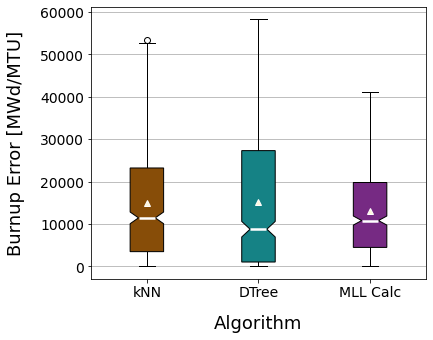
\includegraphics[width=\textwidth]{./chapters/exp1/sfcompo_boxplots_0null_burn.png}
    \caption{Box plots of burnup errors using zero-replaced null values.}
    \label{fig:burn0}
  \end{subfigure}
  \hfill
  \begin{subfigure}[b]{0.49\textwidth}
    \centering
    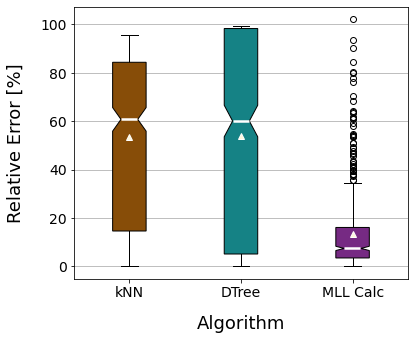
\includegraphics[width=\textwidth]{./chapters/exp1/sfcompo_boxplots_0null_pcterr_burn.png}
    \caption{Box plots of burnup percentage errors using zero-replaced null values.}
    \label{fig:burn0pct}
  \end{subfigure}
  \caption{Box plots of burnup prediction errors and percentage errors for each 
           algorithm using two missing entry techniques: imputation with mean 
           values and replacement with zero.}
  \label{fig:sfcoburn}
\end{figure}

The ranges seen for the imputed nulls test set in Figure \ref{fig:burnimppct}
are as large as they are from low burnups ($< 10 GWd/MTU$) being far
overpredicted, since a small number in the denominator will yield a high
percentage error. A large subset of the low burnup cases are \gls{PHWR}s.
Their burnups are also unlikely to be predicted well because of the inability
of \gls{PHWR} reactors to be represented accurately with this methodology.
Removing the \gls{PHWR} reactors from the results removes all outliers with
percentage errors larger than 1750\%. That is still a very high relative error,
but there are other low burnup cases in the database.  Removing \gls{PHWR}s
does not significantly alter the zero-nulls results in Figure
\ref{fig:burn0pct}.

The range of percentage errors for the zero-nulls test set in Figure
\ref{fig:burn0pct} tells a different story. There is only one case (an
\gls{MLL} outlier) that is above 100\% error.  While the absolute errors for
the scikit-learn algorithms in Figure \ref{fig:burn0} span a larger range than
their counterparts in Figure \ref{fig:burnimp}, their relative errors remain
within $0-100\%$. The only case that predicts the burnup well is the \gls{MLL}
method with the zero-null missing values treatment of the \gls{SFCOMPO} test
set, but about 8\% of the test cases are outliers.  If the best-case median
error of $1.7 GWd/MTU$ in Table \ref{tbl:sfcoburn} were to also correspond to a
lower relative error, then that would be an acceptable result.  However, while
the \gls{MLL} calculations have a percentage error below 20\% at the 75\%
quartile, the non-outlier data reaches almost 40\% and the 8\% of the data
reaches 100\%.

Overall, the absolute errors in Table \ref{tbl:sfcoburn} tell a much more
encouraging story than the box plots in Figure \ref{fig:sfcoburn}, so
investigating beyond the mean and median absolute errors was necessary to show
the real picture of this unique testing scenario. 

\noindent \textbf{\gls{U235} Enrichment}

For both reactor type classification and burnup regressoion, the zero-nulls
test set predicted by \gls{MLL} calculations far outperform all other
algorithm/test set scenarios. However, the enrichment regression results break
this trend.  Table \ref{fig:sfcoenri} shows that decision trees outperform the
other methods, and furthermore, there isn't a large difference in performance
between the two test sets, expecially seeing that the median absolute error is
the same for both test sets.  The other two algorithms follow their previous
behavior: moving from imputed nulls to zero-nulls, \textit{k}-nearest neighbors
has worse performance and \gls{MLL} calculations has better performance.

\begin{table}[!htb]
  \centering
  \begin{tabular}{@{}m{1.5in}llllll@{}}
    \toprule
                     & \multicolumn{3}{m{2in}}{Mean Errors [\% U235]} & \multicolumn{3}{l}{Median Errors [\% U235]} \\ \toprule
    Null Handling    & kNN           & DTree          & MLL          & kNN            & DTree          & MLL    \\ \midrule
    Imputed Nulls    & 0.72          & 0.31           & 1.25         & 0.50           & 0.22           & 1.13   \\
    Zero-value Nulls & 1.67          & 0.36           & 0.49         & 2.02           & 0.22           & 0.35   \\ \bottomrule
  \end{tabular}
  \caption{Mean and median errors for enrichment prediction of the \gls{SFCOMPO} 
           test cases.}
  \label{tbl:sfcoenri}
\end{table}

The mean and median absolute errors are also visible with more statistical
information in the box plots in Figure \ref{fig:sfcoenri}. The outliers for
decision trees and \gls{MLL} calculations are 30 and 16 for the imputed nulls
in Figure \ref{fig:enriimp}, respectively. So although decision trees provides
a typically low absolute error, the outliers reach nearly as far as the spread
of \textit{k}-nearest neighbors. The number of outliers for the zero-nulls
results in Figure \ref{fig:enri0} are 45 and 16 for decision trees and
\gls{MLL} calculations, respectively.  The spread of the outliers for these
algorithms is similar to the previous figure, but \textit{k}-nearest neighbors
has a larger spread of absolute error.

\begin{figure}[!htb]
  \centering
  \begin{subfigure}[b]{0.49\textwidth}
    \centering
    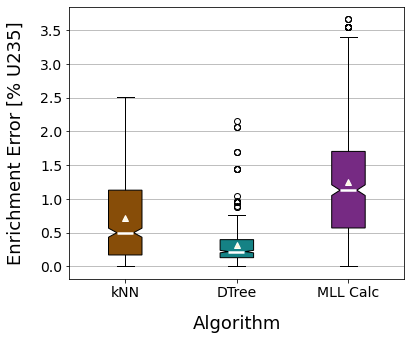
\includegraphics[width=\textwidth]{./chapters/exp1/sfcompo_boxplots_impnull_enri.png}
    \caption{Box plots of enrichment errors using mean-imputed null values.}
    \label{fig:enriimp}
  \end{subfigure}
  \hfill
  \begin{subfigure}[b]{0.49\textwidth}
    \centering
    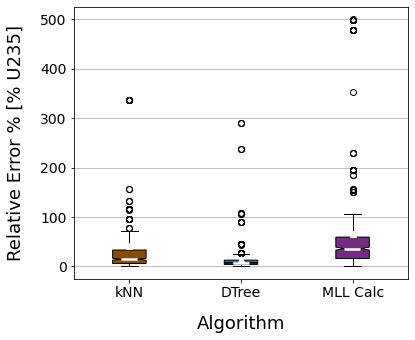
\includegraphics[width=\textwidth]{./chapters/exp1/sfcompo_boxplots_impnull_pcterr_enri.png}
    \caption{Box plots of enrichment percentage errors using mean-imputed null values.}
    \label{fig:enriimppct}
  \end{subfigure}
  \vskip\baselineskip
  \begin{subfigure}[b]{0.49\textwidth}
    \centering
    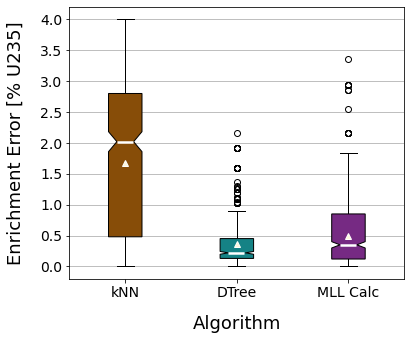
\includegraphics[width=\textwidth]{./chapters/exp1/sfcompo_boxplots_0null_enri.png}
    \caption{Box plots of enrichment errors using zero-replaced null values.}
    \label{fig:enri0}
  \end{subfigure}
  \hfill
  \begin{subfigure}[b]{0.49\textwidth}
    \centering
    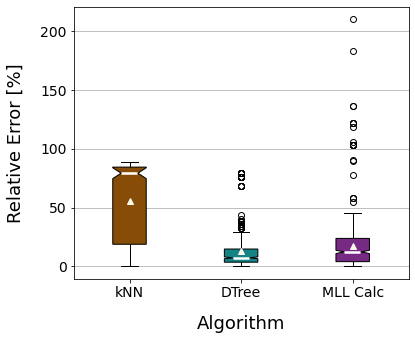
\includegraphics[width=\textwidth]{./chapters/exp1/sfcompo_boxplots_0null_pcterr_enri.png}
    \caption{Box plots of enrichment percentage errors using zero-replaced null values.}
    \label{fig:enri0pct}
  \end{subfigure}
  \caption{Box plots of enrichment prediction errors and percentage errors for 
           each algorithm using two missing entry techniques: imputation with 
           mean values and replacement with zero.}
  \label{fig:sfcoenri}
\end{figure}

Again, a look at the relative errors gives a different sense of these results.
Figures \ref{fig:enriimppct} and \ref{fig:enri0pct} present the percent error
statistics for the imputed nulls and zero-nulls test sets, respectively.  In
Figure \ref{fig:enriimppct} there are 57, 39, and 49 outliers for the
\textit{k}-nearest neighbors, decision trees, and \gls{MLL} calculations,
respectively.  In Figure \ref{fig:enri0pct} there are 44 and 23 outliers for
the decision trees and \gls{MLL} calculations, respectively.

As with the burnup regression, the high percentage errors are caused by a large
overprediction of enrichments that are of low value. All of the \gls{PHWR}s fit
into this category, and removing them from the results removes the outliers
with the highest errors from the imputed nulls results in Figure
\ref{fig:enriimppct}, leaving a maximum of 250\% enrichment error. This is
still a high maximum error because there are other low enrichments not
belonging to the \gls{PHWR} class that remain overpredicted.  As with the
burnup, removing \gls{PHWR}s does not significantly alter the zero-nulls
results in Figure \ref{fig:enri0pct}.

Unlike the case with burnup, the decision trees algorithm gives a better
performance that is null handling-independent than the other algorithm/test set
scenarios. Although there was a slightly worse mean absolute error for the
zero-nulls test set (the median absolute error was the same), the relative
error remains below 100\% for all outliers, as seen in Figure
\ref{fig:enri0pct}.  This makes the decision trees algorithm with the
zero-nulls test set the best performing case for enrichment regression.

It is again true that investigating relative error statistics alongside
absolute error statistics provides a fuller picture of the regression of the
\gls{SFCOMPO} database entries.  It is an unexpected result to have either one
of the scikit algorithms outperform \gls{MLL} calculations for the zero-nulls
test set, since they tended to have lower errors using the imputed nulls test
set. 


